\section{Simulation Experiments and Results}

\subsection{Experimental Setup}

The purpose of the simulation experiments is to connect the analytical
equilibria of the chemostat food-chain model with visible long-time dynamics.
All runs use the internally consistent four-dimensional model
\[
\begin{aligned}
\frac{dS}{dt} &= 1-S-f_1(S)x,\\
\frac{dx}{dt} &= x(f_1(S)-D_1)-f_2(x)y,\\
\frac{dy}{dt} &= y(f_2(x)-D_2)-f_3(y)z,\\
\frac{dz}{dt} &= z(f_3(y)-D_3),
\end{aligned}
\]
where \(S\) is the nutrient concentration, \(x\) is the prey population,
\(y\) is the first predator, and \(z\) is the top predator. The response
functions are Monod functions,
\[
f_i(u)=\frac{a_i u}{k_i+u}, \qquad i=1,2,3.
\]
This version of the system is the one used in the equilibrium and Jacobian
analysis. It was also used by the simulator so that the numerical experiments
and the theoretical formulas describe the same model.

The trajectories were computed with the classical fourth-order Runge--Kutta
method using time step \(\Delta t=0.01\). The initial condition was fixed at
\[
(S_0,x_0,y_0,z_0)=(0.5,0.2,0.1,0.05)
\]
for all five main experiments. The four equilibrium scenarios \(P_0\) through
\(P_3\) were integrated until \(t=500\). The oscillatory case was integrated
until \(t=2000\), because its transient oscillations decay slowly and a shorter
run could give a misleading classification. The simulator wrote every tenth
time step to CSV files and recorded diagnostics including final states,
componentwise minima and maxima, negative-state clamps, explosion status, and
distances from the analytical equilibria. No run exploded and no run required
negative-state clamping.

\begin{figure}[htbp]
    \centering
    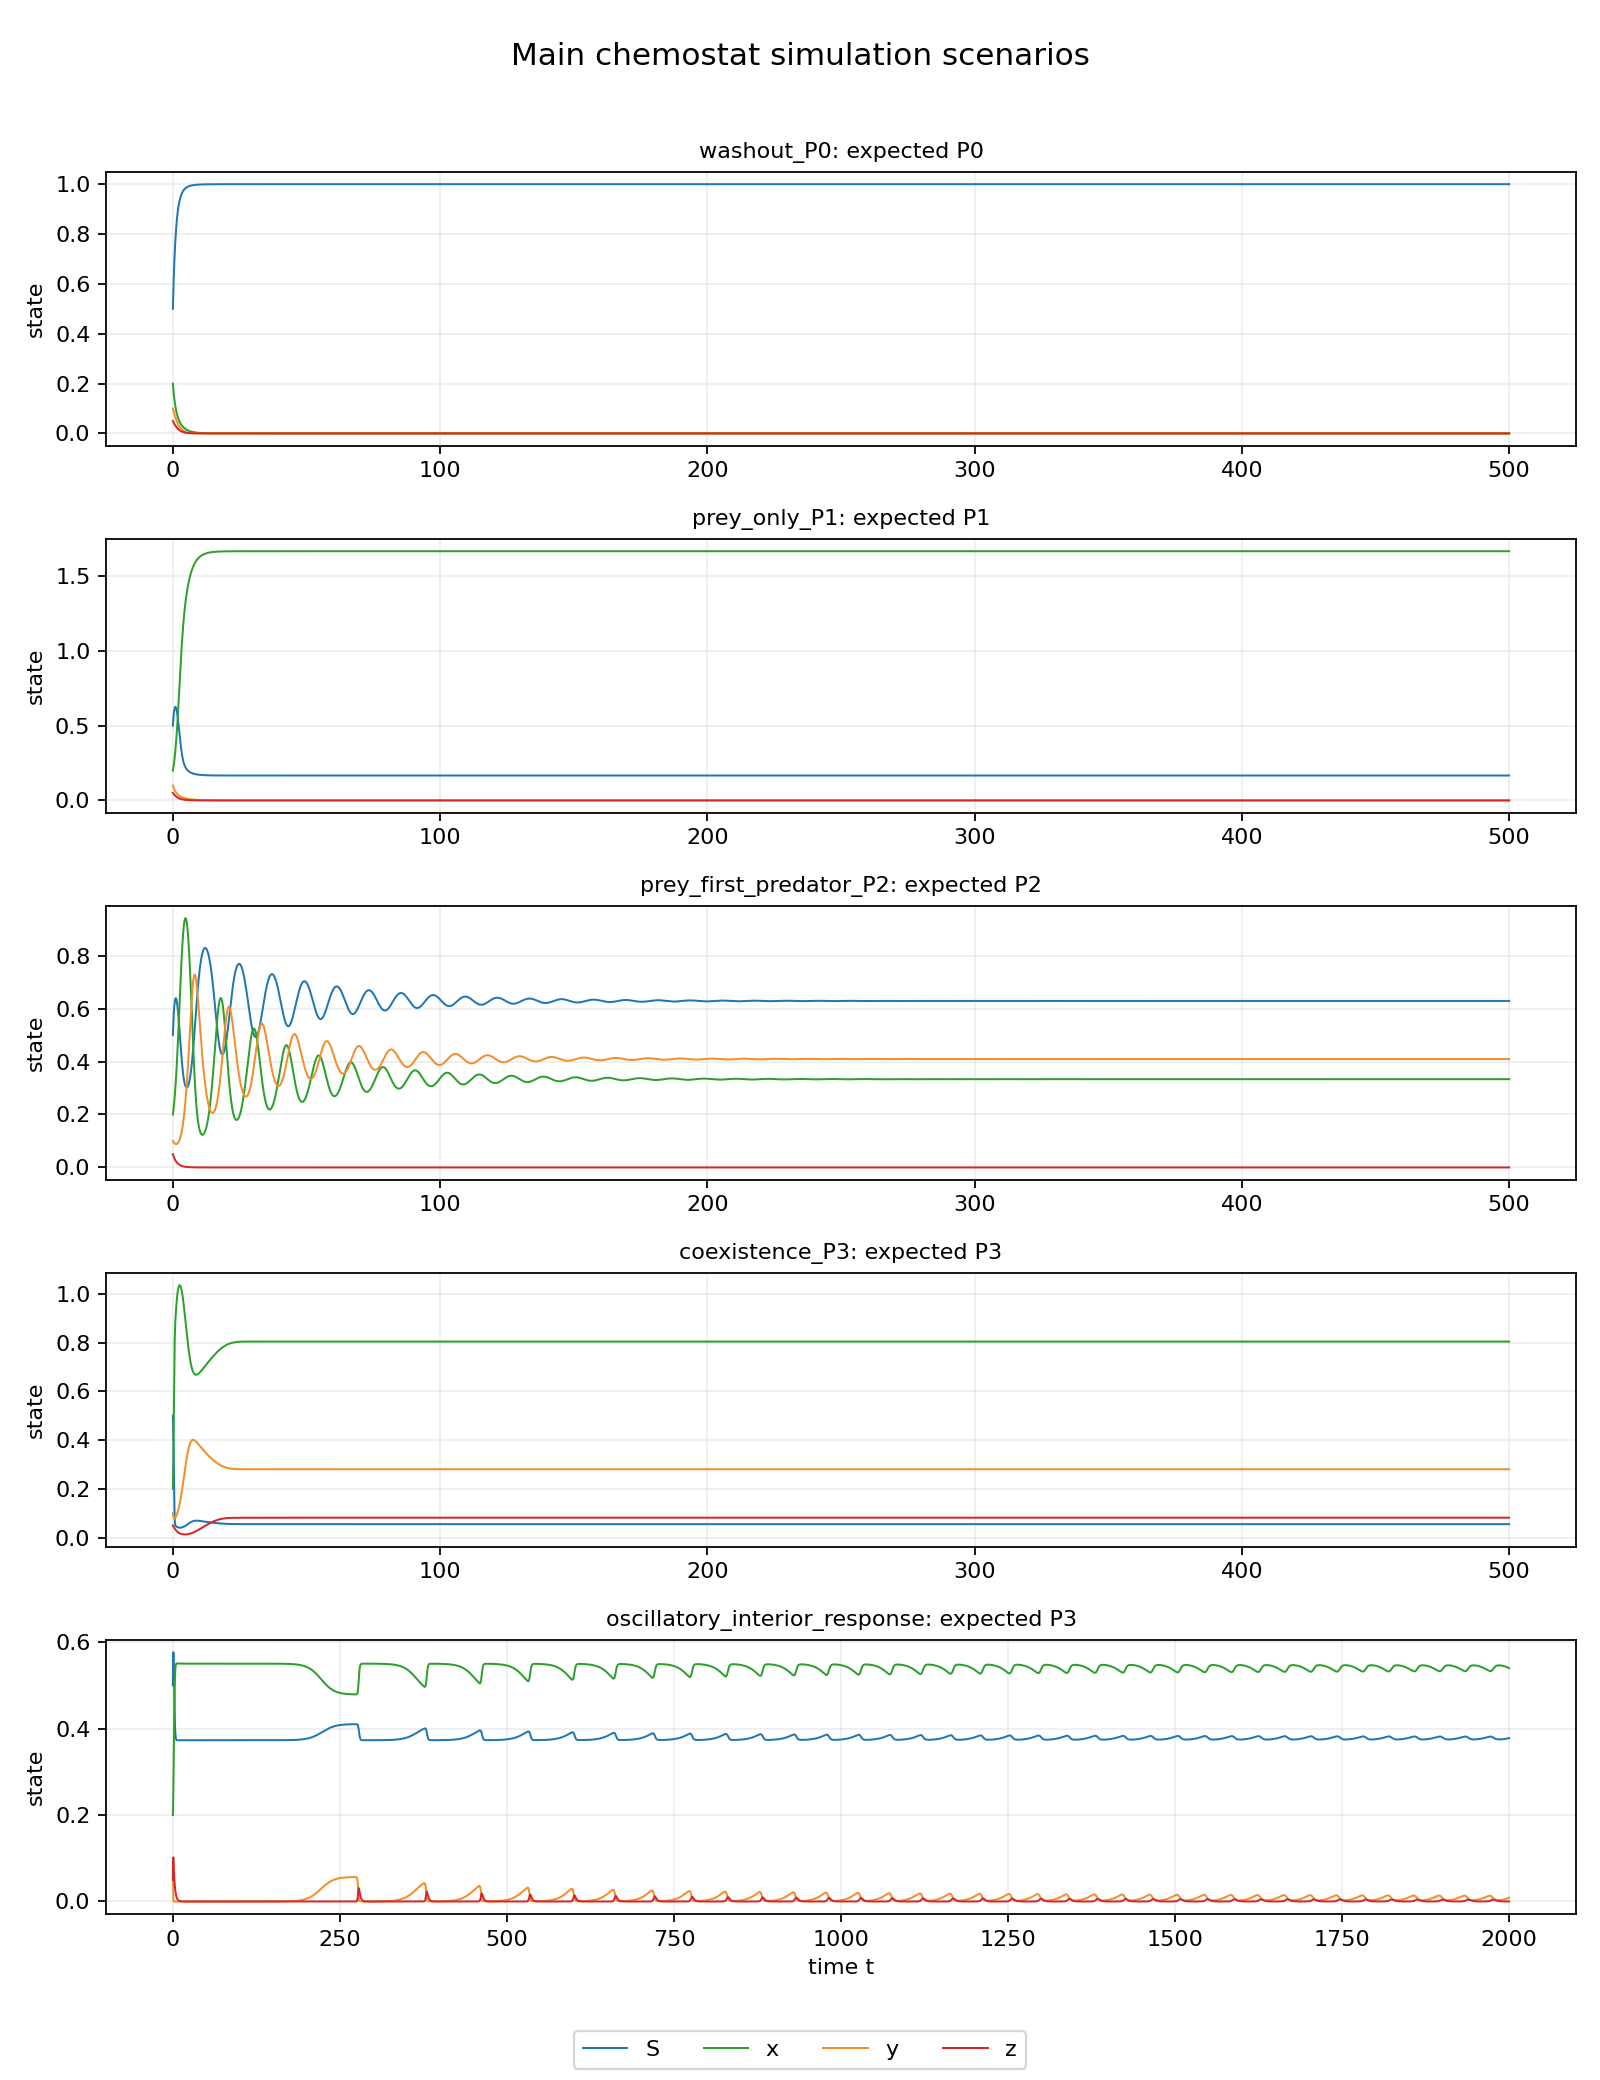
\includegraphics[width=0.95\textwidth]{results/main_scenarios/main_scenarios_overview.png}
    \caption{Overview of the five main simulation regimes generated by the RK4 simulator.}
    \label{fig:main-scenarios-overview}
\end{figure}

\subsection{Parameter-Set Selection}

Five parameter sets were selected to represent the main biological regimes
predicted by the equilibrium hierarchy: complete washout \(P_0\), prey-only
survival \(P_1\), survival of the prey and first predator \(P_2\), coexistence
of all trophic levels \(P_3\), and a slowly damped oscillatory response near
an interior equilibrium. The values used in the simulations are listed in
Table~\ref{tab:main-scenario-parameters}.

\begin{table}[htbp]
\centering
\caption{Parameter sets used in the main simulation experiments.}
\label{tab:main-scenario-parameters}
\resizebox{\textwidth}{!}{%
\begin{tabular}{lccccccccc}
\hline
Scenario & \(a_1\) & \(k_1\) & \(a_2\) & \(k_2\) & \(a_3\) & \(k_3\) & \(D_1\) & \(D_2\) & \(D_3\)\\
\hline
\(P_0\) washout & 0.60 & 0.50 & 1.50 & 0.50 & 1.20 & 0.40 & 0.80 & 0.70 & 0.70\\
\(P_1\) prey only & 2.00 & 0.50 & 0.50 & 1.00 & 1.00 & 1.00 & 0.50 & 0.60 & 0.60\\
\(P_2\) two species & 2.00 & 0.50 & 2.00 & 1.00 & 0.50 & 1.00 & 0.50 & 0.50 & 0.70\\
\(P_3\) coexistence & 4.80 & 0.17 & 4.30 & 1.85 & 4.60 & 1.66 & 0.72 & 1.11 & 0.665\\
Oscillatory response & 6.52 & 1.76 & 5.07 & 2.64 & 3.78 & 0.0466 & 1.14 & 0.778 & 0.488\\
\hline
\end{tabular}%
}
\end{table}

\subsection{Washout Scenario P0}

In the washout scenario, the numerical solution converged to
\[
(S,x,y,z)\approx(1,0,0,0),
\]
with distance \(5.55\times 10^{-15}\) from the analytical equilibrium \(P_0\).
Biologically, this means that the prey cannot grow fast enough on the incoming
nutrient to overcome its removal rate. Once the prey disappears, both predator
populations also disappear because their food sources are absent. The nutrient
therefore returns to its normalized input concentration.

\begin{figure}[htbp]
    \centering
    
\includegraphics[width=0.88\textwidth]{results/main_scenarios/washout_P0_timeseries.png}
    \caption{Running simulation image for the washout scenario \(P_0\).}
    \label{fig:washout-p0-timeseries}
\end{figure}

\subsection{Prey-Only Scenario P1}

In the prey-only scenario, the final numerical state was
\[
(S,x,y,z)\approx(0.166667,1.666667,0,0),
\]
with distance \(2.57\times 10^{-14}\) from the theoretical equilibrium \(P_1\).
The prey population survives because it can exploit the nutrient supply, but
the resulting prey concentration is not sufficient for the first predator to
overcome its own removal rate. Consequently both predators wash out. The
nutrient level is much lower than in \(P_0\), showing that prey persistence is
associated with continuous nutrient consumption.

\begin{figure}[htbp]
    \centering
    
\includegraphics[width=0.88\textwidth]{results/main_scenarios/prey_only_P1_timeseries.png}
    \caption{Running simulation image for the prey-only scenario \(P_1\).}
    \label{fig:prey-only-p1-timeseries}
\end{figure}

\subsection{Two-Species Scenario P2}

In the two-species scenario, the solution approached
\[
(S,x,y,z)\approx(0.628666,0.333334,0.409333,0),
\]
which is \(1.29\times 10^{-6}\) from the analytical equilibrium \(P_2\). The
prey and first predator persist, while the top predator is removed from the
system. This confirms the expected intermediate regime in which the first
predator can invade the prey-only equilibrium, but the second predator cannot
invade the prey--predator equilibrium. The approach to \(P_2\) contains small
damped transients, so temporary oscillation should not be confused with
sustained periodic behavior.

\begin{figure}[htbp]
    \centering
    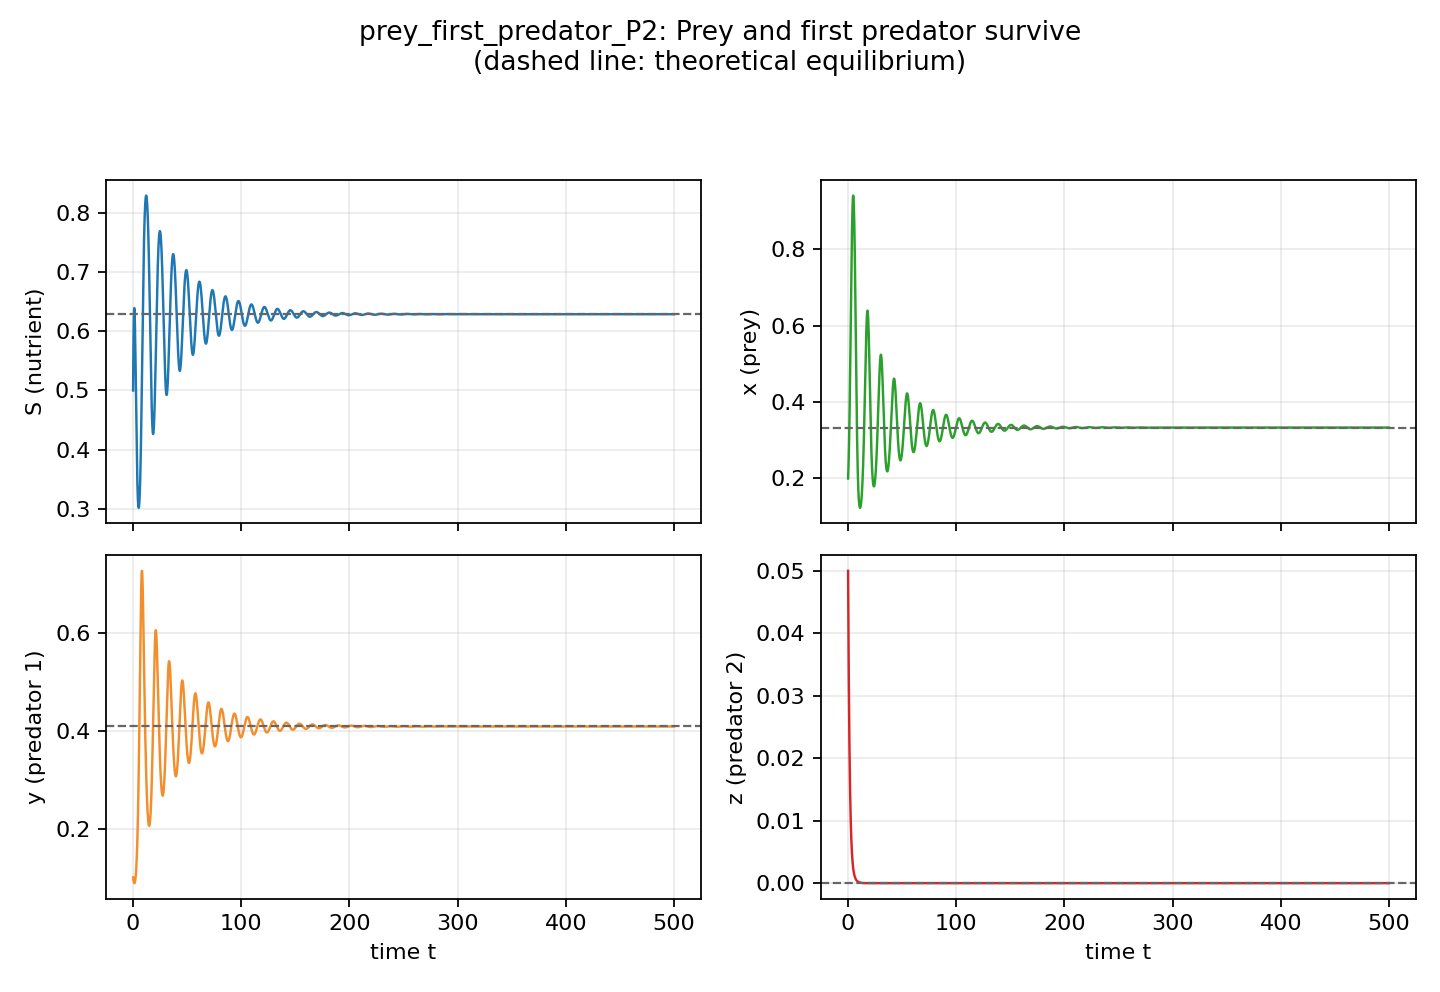
\includegraphics[width=0.88\textwidth]{results/main_scenarios/prey_first_predator_P2_timeseries.png}
    \caption{Running simulation image for the two-species scenario \(P_2\).}
    \label{fig:two-species-p2-timeseries}
\end{figure}

\subsection{Coexistence Scenario P3}

In the coexistence scenario, all state variables converged to positive values:
\[
(S,x,y,z)\approx(0.055067,0.804597,0.280534,0.081550).
\]
The distance from the analytical coexistence equilibrium \(P_3\) was
\(1.94\times 10^{-11}\). This close agreement shows that the simulator
reproduces the expected interior equilibrium for the selected parameter set.
In biological terms, nutrient enters the chemostat continuously, the prey
consumes nutrient, the first predator consumes prey, and the top predator
consumes the first predator. This numerical result supports the persistence
interpretation in the reference, although a single trajectory is not a proof
of uniform persistence for all admissible positive initial conditions.

\begin{figure}[htbp]
    \centering
    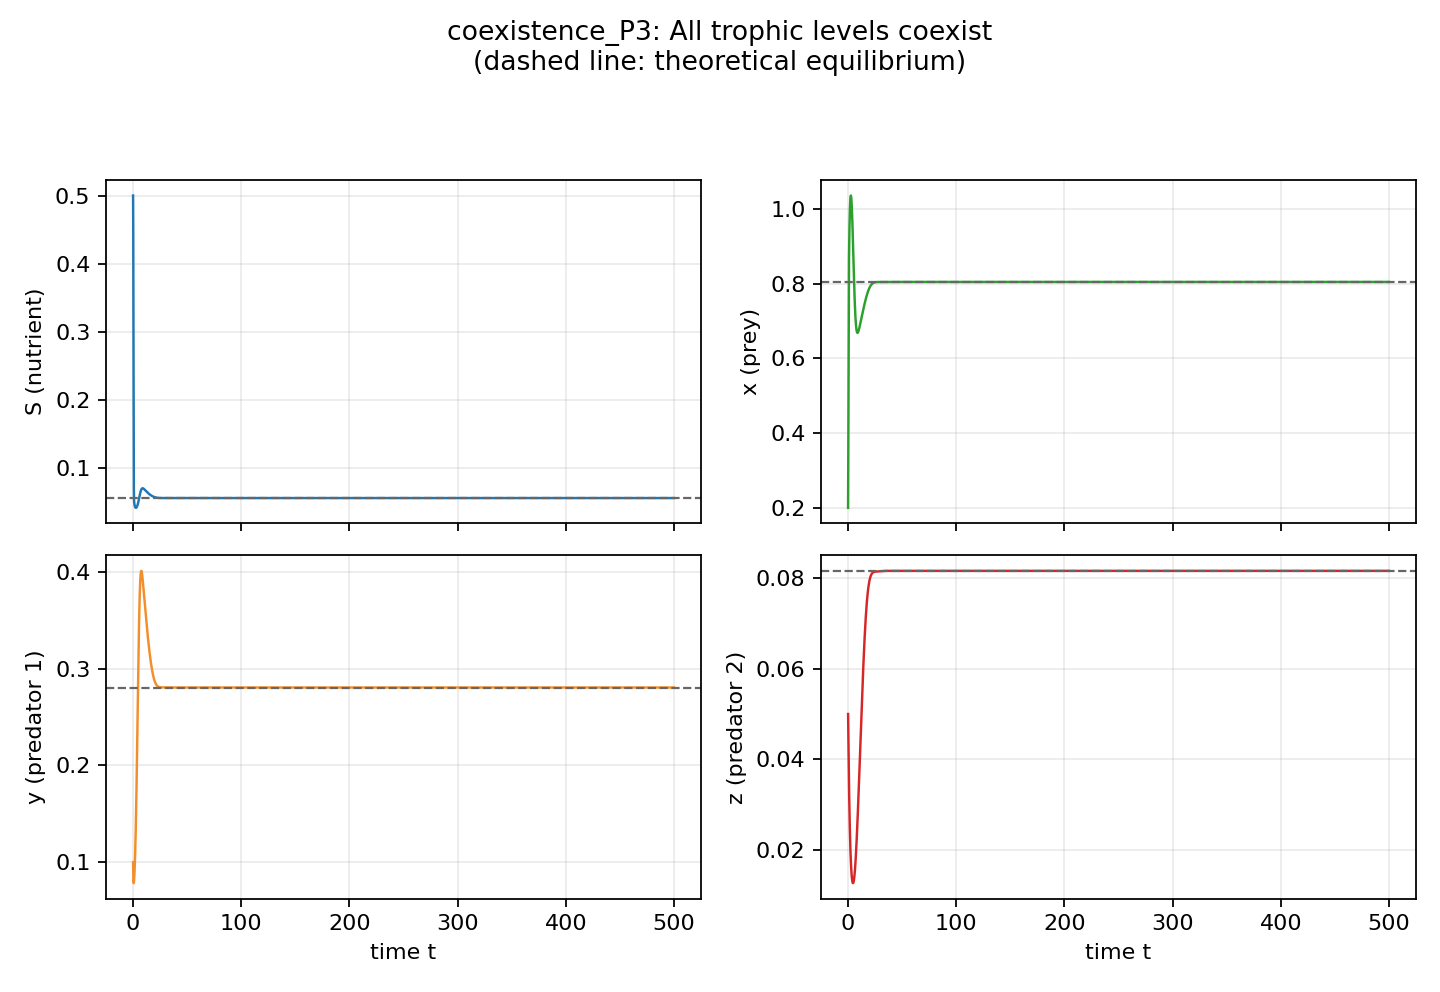
\includegraphics[width=0.88\textwidth]{results/main_scenarios/coexistence_P3_timeseries.png}
    \caption{Running simulation image for the coexistence scenario \(P_3\).}
    \label{fig:coexistence-p3-timeseries}
\end{figure}

\subsection{Oscillatory and Damped-Oscillatory Response}

The fifth scenario was included to demonstrate an interior response with
visible oscillations. Its analytical target equilibrium is
\[
P_3=(0.377311,0.540994,0.006908,0.001193).
\]
At \(t=2000\), the instantaneous numerical state was
\[
(S,x,y,z)\approx(0.377832,0.539609,0.008618,0.000146),
\]
with distance \(2.49\times 10^{-3}\) from \(P_3\). This final-state distance is
larger than in the previous cases because the endpoint depends on the phase of
the remaining oscillation.

To avoid misclassification, the oscillatory case was also evaluated using
window statistics. Over the late window \(1500\leq t\leq 2000\), the mean state
was only \(4.66\times 10^{-4}\) from \(P_3\). After \(t=500\), the trajectory
had 23 detected local maxima in \(y\) and 20 detected local maxima in \(z\).
The maximum ratio between the late-window amplitude and the middle-window
amplitude was 0.425, so the oscillations were decreasing. These measurements
identify the behavior as a slowly damped oscillatory approach to the interior
equilibrium. They are consistent with dynamics near a Hopf stability boundary,
but they do not by themselves prove a Hopf bifurcation.

\begin{figure}[htbp]
    \centering
    
\includegraphics[width=0.88\textwidth]{results/main_scenarios/oscillatory_interior_response_timeseries.png}
    \caption{Running simulation image for the slowly damped oscillatory scenario.}
    \label{fig:oscillatory-timeseries}
\end{figure}

\begin{figure}[htbp]
    \centering
    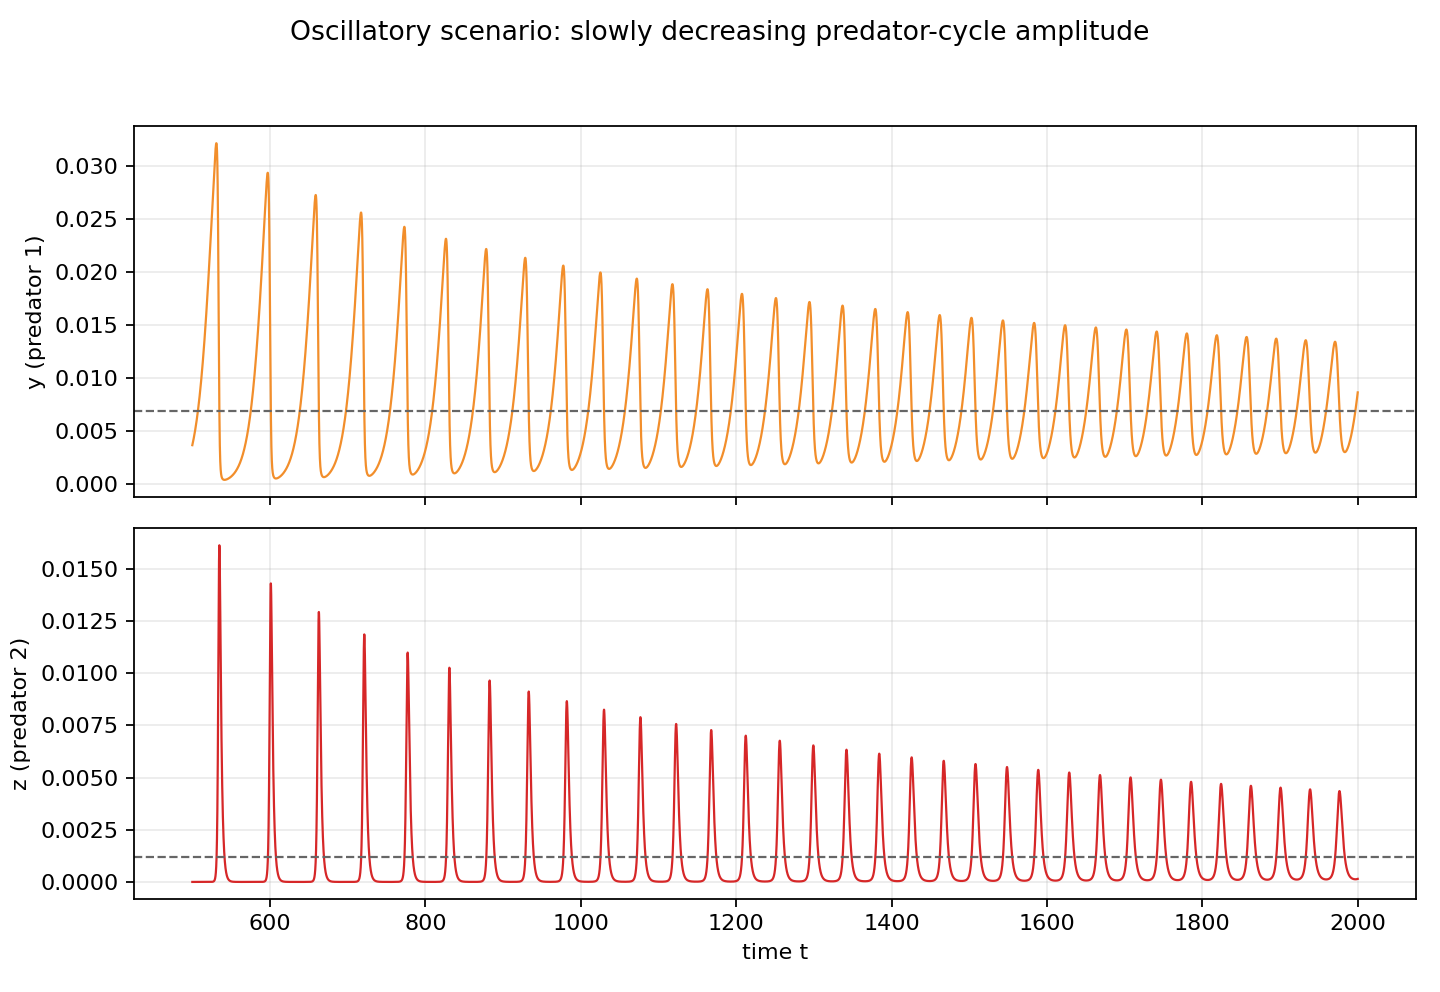
\includegraphics[width=0.88\textwidth]{results/main_scenarios/oscillatory_interior_response_zoom.png}
    \caption{Zoomed view of the predator oscillations after the initial transient.}
    \label{fig:oscillatory-zoom}
\end{figure}

\subsection{Comparison Between Numerical and Theoretical Equilibria}

Table~\ref{tab:numerical-theoretical-comparison} compares the numerical final
states with their theoretical targets. The first four experiments agree with
their expected equilibria to high accuracy. The oscillatory case is naturally
less well represented by a single final point, so its window average was used
as the main evidence for convergence toward \(P_3\).

\begin{table}[htbp]
\centering
\caption{Comparison between numerical final states and theoretical equilibria.}
\label{tab:numerical-theoretical-comparison}
\begin{tabular}{lllc}
\hline
Scenario & Target & Numerical final state \((S,x,y,z)\) & Distance\\
\hline
\(P_0\) washout & \(P_0\) & \((1.000000,0,0,0)\) & \(5.55\times 10^{-15}\)\\
\(P_1\) prey only & \(P_1\) & \((0.166667,1.666667,0,0)\) & \(2.57\times 10^{-14}\)\\
\(P_2\) two species & \(P_2\) & \((0.628666,0.333334,0.409333,0)\) & \(1.29\times 10^{-6}\)\\
\(P_3\) coexistence & \(P_3\) & \((0.055067,0.804597,0.280534,0.081550)\) & \(1.94\times 10^{-11}\)\\
Oscillatory response & \(P_3\) & \((0.377832,0.539609,0.008618,0.000146)\) & \(2.49\times 10^{-3}\)\\
\hline
\end{tabular}
\end{table}

\subsection{Biological Interpretation of the Results}

The simulations show a clear trophic survival hierarchy. In \(P_0\), the prey
cannot overcome removal, so the entire biological chain washes out. In \(P_1\),
the prey survives but does not create enough food supply for predators. In
\(P_2\), the first predator persists, but the top predator cannot invade. In
\(P_3\), all trophic levels have sufficient effective growth relative to their
removal rates, so the system settles at a positive coexistence equilibrium.

The main biological mechanism is therefore the balance between food-dependent
growth and species-specific removal. Each higher trophic level can persist
only if the lower level maintains a concentration high enough to make the
corresponding Monod response exceed the removal rate. The numerical results
also show why long simulations and analytical equilibria should be used
together. Graphs reveal transient oscillations, while equilibrium distances
give a quantitative test of the predicted long-term regime.

\subsection{Interactive Simulator Demonstration}

The project also includes an interactive browser simulator in the
\texttt{demo/} directory. It can be launched from the repository root by
running
\[
\texttt{python -m demo.app}
\]
and then opening \(\texttt{http://127.0.0.1:8000}\) in a browser. The
interface allows the user to choose scenario presets, change the removal
rates \(D_1,D_2,D_3\), adjust the Monod parameters, and observe the RK4
trajectory in real time. It also displays analytical equilibria, invasion
thresholds, local stability information, and the nearest equilibrium to the
current live state. This makes the simulation results easier to interpret
during the presentation because the audience can see how changing a removal
rate moves the system between washout, partial survival, and coexistence.

\begin{figure}[htbp]
    \centering
    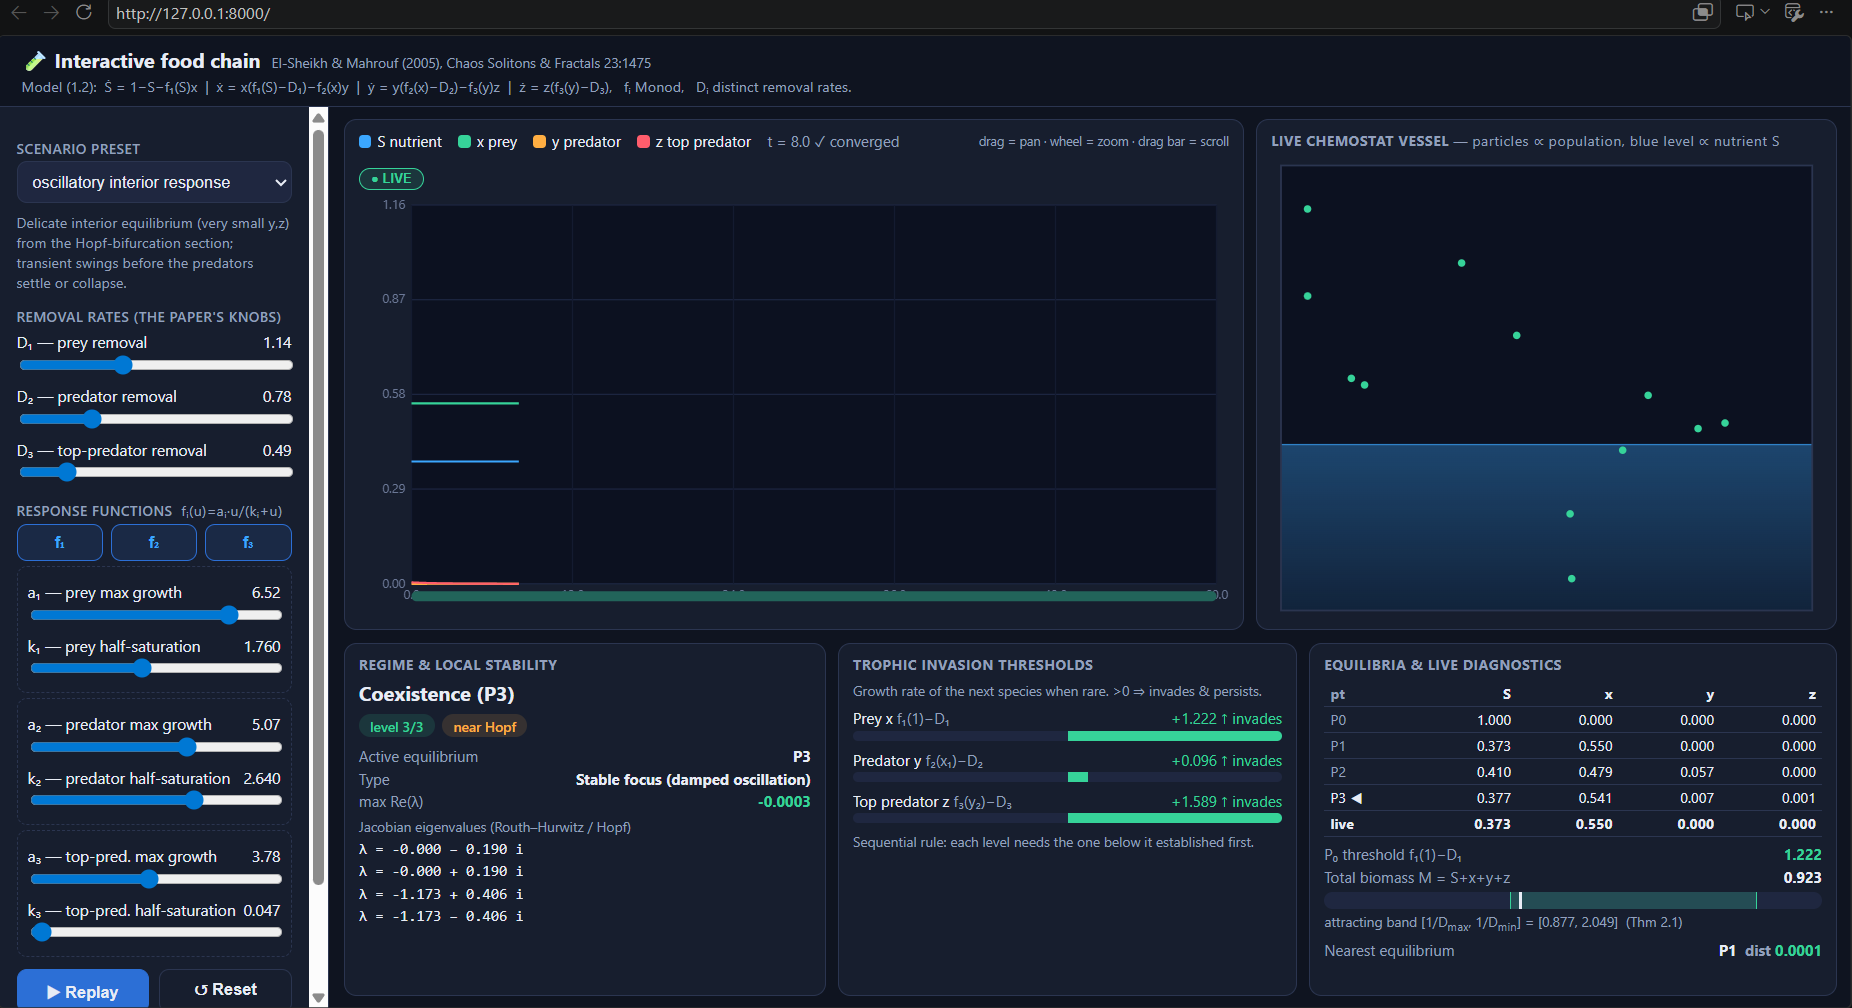
\includegraphics[width=1\textwidth]{images/UI.png}
    \caption{Screenshot of the interactive simulator showing live trajectories, parameter sliders, equilibrium table, and stability diagnostics.}
    \label{fig:interactive-simulator-demo}
\end{figure}
